\documentclass{article}
\usepackage{graphicx}
\usepackage{hyperref}
\usepackage{amsmath}

% Title content
\title{Transferability of Adversarial Reinforcement Learning}
\author{Connor Fuhrman, Johnathan Gill}
\date{May 11 2021}

\begin{document}

\maketitle

\begin{abstract}
It is well known that deep learning and deep reinforcement learning (RL) are vulnerable to adversarial attacks via a model's observations. 
Recently, it was shown that RL is susceptible to adversarial attacks on the \textit{policy} alone via an attacker trained to develop an adversarial policy. 
Such attacks are especially interesting because the adversarial attacker does not simply perturb the victim's model's input, i.e., in RL the observation space, but rather choses physically realistic actions such that the victim's policy breaks down. 
This method of adversarial attack is especially interesting because real-world RL agents may only interact with each other and the environment around them in a physically realistic fashion. 
This work investigates the transferability of such adversarial policies between various model architectures via a "shoot and defend" type game. 
Quadcopter agents are trained to be either the shooter, who's goal is to shoot a ball into a goal, or a defender, who's goal is to keep the ball out of the goal. 
There are two shooter agents trained with varying model architectures and two keeper agents, one of which is trained adversarially against one shooter agent but \texttt{not} the other. 
We find that ...
\end{abstract}

\newpage

\section{Introduction}\label{sec:intro}
Adversarial attacks against neural network classifiers \cite{Szegedy2014} and (deep) reinforcement learning (RL) \cite{Gleave2019} has been shown effective via adversarial perturbations of the victim model's input, e.g., altering pixel values for an image classifier or perturbing an observation space for an RL model. 
However, such attacks are artificial when considering real-world RL agents as an adversarial attacker cannot directly alter image pixel or observation space values but can only interact naturally with the environment and the victim model, e.g., an adversarial attack against an autonomous unmanned aerial vehicle (UAV) cannot access the UAV's perception equipment directly to alter measurement values nor can it alter the environment in a non-physically realistic manner. 
\\
\noindent 
Work done in \cite{Gleave2019} showed that an adversarial policy was effective in multiple zero-sum games, including shoot and defend where the \textit{shooter} agent attempts to shoot a ball into a goal while the \textit{keeper} agent seeks to keep the ball out of the goal. 
The adversarial attacker, the keeper agent, demonstrated significantly different activations than the normal models and was overall successful in each game by manipulating only it's own body position to exploit weaknesses in the victim's (the shooter agent) policy.
Videos showing the results from \cite{Gleave2019} are available \href{https://adversarialpolicies.github.io/}{online} and show that adversarial policies are more effective in higher-dimensional spaces such as humanoid models over lower-dimensional spaces such as ants. 

\begin{figure}[h!]
  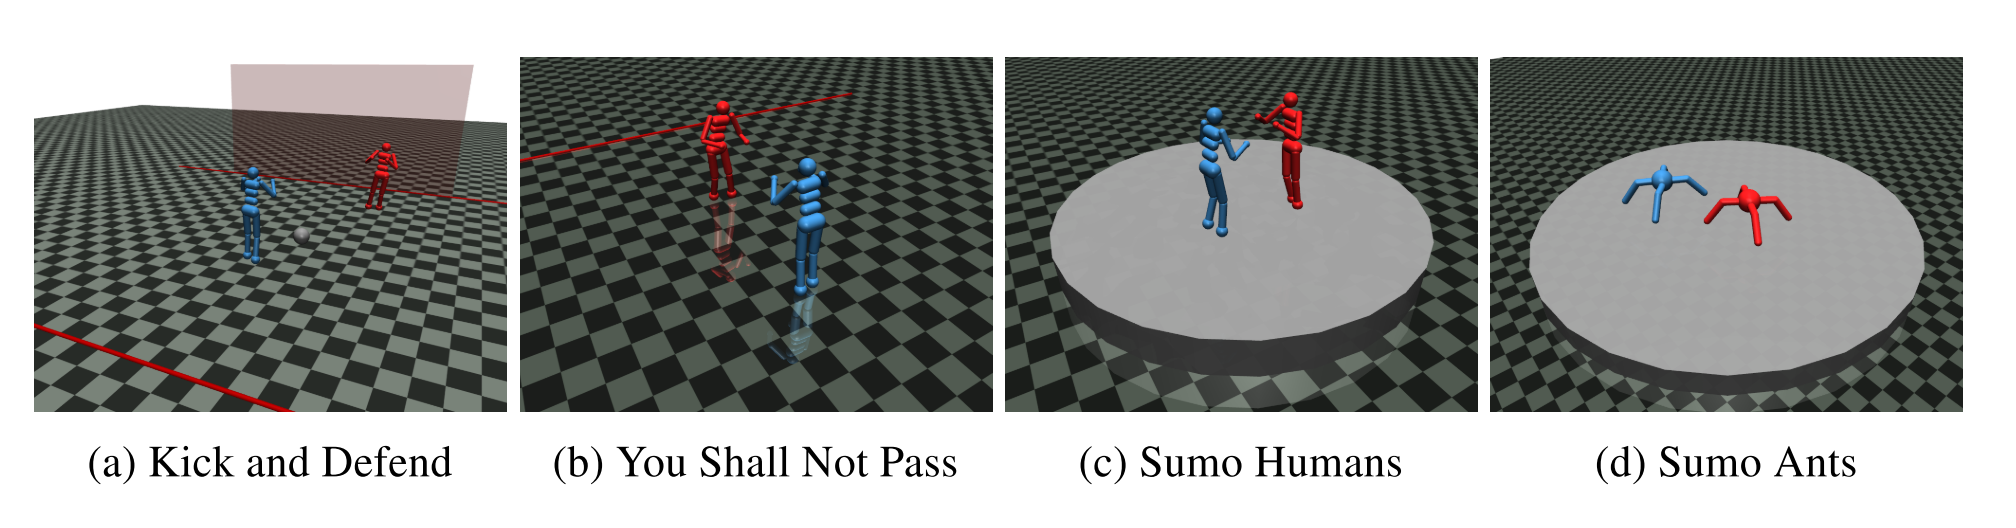
\includegraphics[width=\linewidth]{imgs/Gleave2019_env}
  \caption{Training environment used in \cite{Gleave2019} showing all four zero-sum games investigated for adversarial policies}
  \label{fig:gleave_env}
\end{figure}

\noindent 
The adversarial agents in \cite{Gleave2019} were given unlimited black-box access to the victim's policy, $\pi_v$, but were not given any white-box access to model weights or activations. 
The victim model's policy was frozen and actions were sampled from the stochastic policy such that $a_v$ is a sample of the stochastic policy $\pi_v(. | s)$ while the adversary developed a policy $\pi_a$ such that $\pi_a$ maximizes the discounted sum of rewards. 
Agents trained adversarially demonstrate reliable domination of the vicim models, winning upwards of 90\% of games in most cases. 
However, it is interesting to note that when the victim is "blind" to the attacker, i.e., the victim's observations corresponding to the attacker's position is set statically to a typical initial value, its performance increases significantly from losing over 80\% of games to winning 99\% of games in \textit{You Shall Not Pass} (this game demonstrates the phenomenon best but the trend exists in other games). 

\section{Methods}\label{sec:methods}
The following sections discuss the gym environment, RL framework, and deployment on the high performance computing (HPC) cluster at the University of Arizona.

\subsection{Gym Environment}\label{subsec:gym_env}
We utilize an OpenAI-based gym environment introduced in \cite{Panerati2021} which provides a multi-agent RL environment based on the \texttt{Bullet} physics engine. 
The environment, \texttt{gym-pybullet-drones}, (original repository available online at \url{github.com/utiasDSL/gym-pybullet-drones}) allows users to rapidly create new environments and instantiate models within defined by their Unified Robot Description Format (URDF). \\

\noindent
The drone model utilized in this work is the \href{https://www.bitcraze.io/documentation/hardware/crazyflie_2_1/crazyflie_2_1-datasheet.pdf}{Bitcraze Cracyflie 2.1} as this model ships with the gym environment. 
The quadcopter itself is a small open-source development platform which weight under 30g and is intended for education, research, and in particular swarm applications. 
Note, however, that this model in particular are not integral to this work but was chosen simply because they were readily available.

\subsection{Shoot and Defend Environment}\label{subsec:sad_env}
The \textit{Shoot and Defend} environment is configured as in Figure~\ref{fig:sad_env}. 
\begin{figure}[t!]
  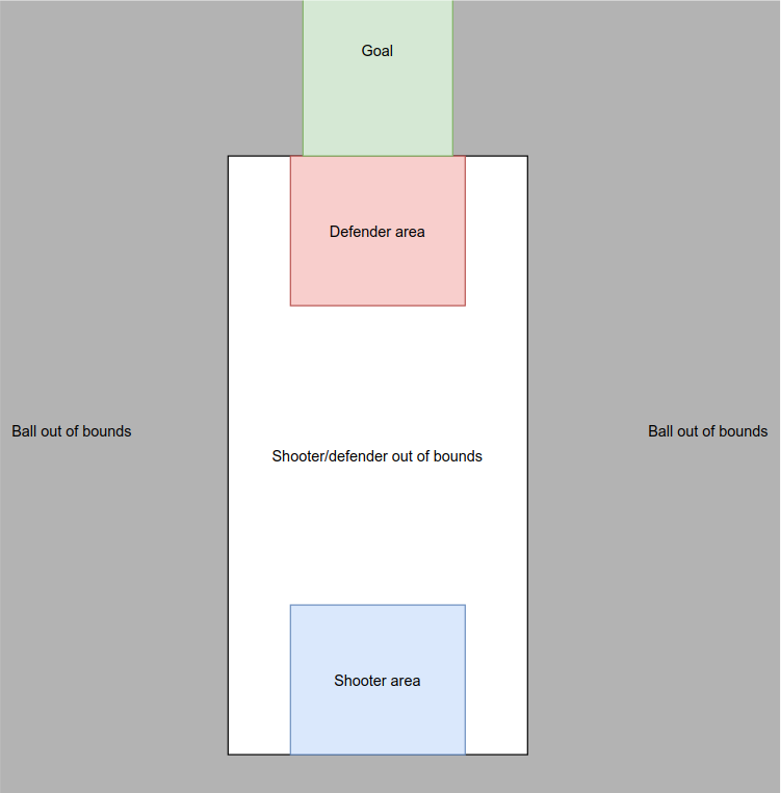
\includegraphics[width=\linewidth]{imgs/ShootAndDefend_env}
  \caption{Diagram depicting the \textit{Shoot and Defend} environment. Note this is a top-down view as the shooter and defender may travel in the vertical direction.}
  \label{fig:sad_env}
\end{figure}
The shooter and defender agents are each constrained to remain in their respective areas and recivee a punishment if this boundary is violated. 
The shooter agent receives a reward if the ball enters the goal area and a penalty if the ball goes out of bounds or becomes stationary. 
Both agents also receive penalties for crashing and other undesirable behavior. 
The exact rewards and conditions are shown in Appendix~\ref{app:rewards}. \\

\noindent
The observation space for each agent is the physical properties of all physical objects in the scene, i.e., the position, attitude, velocity, and angular velocity. 
However, in order to reduce the complexity and without loss of generality the observations for the ball object are simply position and velocity as the ball's attitude and angular velocity \footnote{The ball is shot with a force of 50N and there is no external force applied by moving air. The ball is then essentially only affected by gravity and would not experience a curved trajectory as in a windy environment} do not play as significant a role in the game as the position and velocity. 
Therefore, the dimensionality for the observation space of each agent is a 30-length vector. 
The action space for the defender agent is an 8-vector representing the mean and standard deviation of a Gaussian distribution by which motor revolution per minute (RPM) values are sampled. 
The shooter agent adds an additional mean and standard deviation pair which indicates that the shooter agent should shoot the ball. 
If the value of this sampled distribution is above a threshold, the shooter launches the ball in the drone platform's current orientation \footnote{Note that the ball is instantiated as a model at the time of shooting and the shooter agent does not carry the ball beforehand.}. 

\subsection{Training Methodology}\label{subsec:train_methods}
Both the shooter and defender agents are trained using Proximal Policy Optimization (PPO) \cite{Schulman2017} via the Ray RLlib library \cite{Liang2017} which provides RL-specific libraries and functionality atop the Ray API for distributed operation.
PPO was chosen over, e.g, Q networks, due to its ability to handle continuous action spaces such as the quadcopter's RPM commands. 
Policy gradient methods have been demonstrated to achieve state-of-the-art performance using deep neural networks in multiple application areas including, but not limited to, Go, Atari and other video games, and 3D locomotion \cite{ppo_site}. 
PPO addresses issues with various other policy optimization methods such as sensitivity to step size and poor sample efficiency while avoiding overcomplicated implementations, e.g., Actor-Critic with Experience Replay (ACER) \cite{wang2017sample} which introduces more implementation complexity via off-policy correction and a replay buffer while showing only marginal improvement over PPO in OpenAI's Atari benchmark \cite{ppo_site}, or algorithms which are unable to share parameters between the policy and value function or auxiliary losses such as dropout (e.g., Atari games or other domains heavily-reliant on visual input \cite{ppo_site}), e.g, Trust Region Policy Optimization (TRPO) \cite{schulman2017trust}. 
PPO utilizes the objective function
\begin{equation} \label{eq:ppo_loss}
L^{CLIP}(\theta) = \hat{E}_t[min(r_t(\theta) \hat{A}_t , clip(r_t(\theta), 1-\epsilon, 1+\epsilon) \hat{A}_t]
\end{equation}
where
\begin{itemize}
\item $\theta$ is the policy parameter
\item $\hat{E}_t$ is the empirical expectation over timesteps
\item $r_t$ is the ratio of probabilities under the new and old policies respectively
\item $\hat{A}_t$ is the estimated advantage at time $t$ 
\item $\epsilon$ is a hyperparameter \footnote{The authors of \cite{Schulman2017} and \cite{ppo_site} recommend usually 0.2 or 0.3}
\end{itemize}

\noindent
We utilize the PPO implementation via the Ray RLlib \cite{ray_ppo} as the Ray library provides abstractions for parallelization and distributed workflows and the RLlib library contains a suite of highly parallelizable GPU-enabled algorithms which are (mostly) compatible with both TensorFlow and PyTorch. 

\begin{figure}
  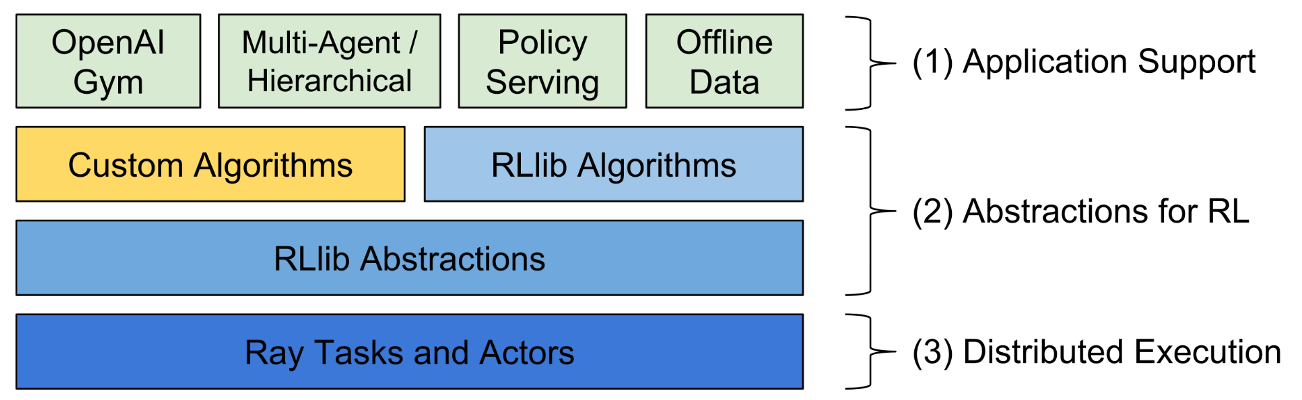
\includegraphics[width=\linewidth]{imgs/ray_blockdiagram}
  \caption{Ray library conceptual block diagram \cite{ray_ppo}. The \textit{Shoot and Defend} environment created herein is an OpenAI-compatible Gym and we utilize RLlib algorithms which utilize Ray's abstraction layer to effectuate distributed execution.}
  \label{fig:ray_blockdiagram}
\end{figure}

\newpage
\appendix
\section{Agent Rewards}\label{app:rewards}
TODO 

\section{Ray PPO Configuration} \label{app:ray_config}
TODO


\newpage
\bibliographystyle{plain}
\bibliography{reference.bib}

\end{document}